\documentclass{paper}
\usepackage[margin=0.5in]{geometry}
\usepackage{graphicx}
\usepackage{listings}

% \includegraphics[scale=1]{img.png}
% \begin{lstlisting} 
\title{2. Memory Protection}
\begin{document}
\maketitle
\begin{large}\textbf{Hvad er memory protection?}\end{large}\\
\line(1,0){510}
\begin{itemize}
	\item Benyttes til at kontrollere rettigheder til forskellige dele af memory
	\item Hovedform\aa let er at forhindre processer i at f\aa\ adgang til dele af memory den ikke har rettigheder til at tilg\aa\
	\item S\o rger blandt andet ogs\aa\ for segmentation faults\\
\end{itemize}

\begin{large}\textbf{Hvordan fungerer en MMU?}\end{large}\\
\line(1,0){510}
\begin{itemize}
	\item Typisk indbygget i CPU'en
	\item S\o rger for at et program afvikles i sin egen private memory space
	\item G\o r virtuel memory mulig, som er uafh\ae ngig af af fysisk memory
	\item MMU'en er en overs\ae tter fra virtuelle adresser til fysiske adresser
	\item Dette muligg\o r at programmer afvikles med de samme virtuelle adresser, mens de faktisk er p\aa\ forskellige fysiske adresser
	\item De virtuelle adresser tildeles af compiler og linker, MMU'en soerger for at allokere dem i den fysiske hukkomelse
	\item En af grundstenene for simplere/organiseret multitasking\\
	\item \textbf{Translation Lookaside Buffer(TLB)}
	\begin{itemize}
		\item Cacher nyeligt tilg\aa ede pages
		\item Benytter main memory til at gemme information om virtelle memory maps(PTE - Page Table Entry)
		\item Indeholder information om fysisk adresse, st\o rrelse, rettigheder, cache\\
	\end{itemize}
\end{itemize}

\begin{large}\textbf{Hvordan laver man context switching vha en MMU?}\end{large}\\
\line(1,0){510}
\begin{enumerate}
	\item Gem den aktivere process' indhold og s\ae t den i dormant state(sleep)
	\item Ryd cache
	\item Ryd TLB
	\item Opdater med den nye process' page tables
	\item Genskab den nye process\\
\end{enumerate}

\begin{large}\textbf{Hvordan benytter Linux sig af en MMU?}\end{large}\\
\line(1,0){510}
\begin{itemize}
	\item Linux kan ikke afvikles uden en MMU
	\item MMU'en s\o rger for opdelingen af kernel-/user-space
	\item Virtuel memory er en hoved del af Linux 
	\item Segmentation faults
	\item Data beskyttelse
\end{itemize}
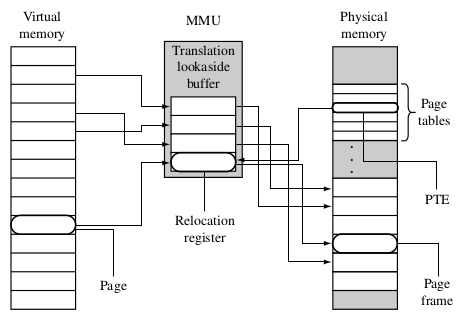
\includegraphics[scale=0.7]{mmu.png}
\end{document}
